\documentclass[10pt,twocolumn,a4paper]{article}
\usepackage[utf8]{inputenc}
\usepackage[T1]{fontenc}
\usepackage{times}
\usepackage[margin=1.8cm,columnsep=0.6cm]{geometry}
\usepackage{graphicx}
\usepackage{booktabs}
\usepackage{amsmath}
\usepackage{xcolor}
\usepackage[hidelinks]{hyperref}
\usepackage{url}
\usepackage{caption}
\captionsetup{font=small,labelfont=bf}
\newcommand{\todo}[1]{\textcolor{red}{[#1]}}

\title{Keeping the Dog, Muting the Human:\\ Speech Removal for Dog--Human Play Recordings}
\author{Nurmuhammed Kanybekov \quad Péter Kovács\\
\small Faculty of Informatics, Eötvös Loránd University (ELTE), Budapest, Hungary\\
\small \todo{draft of 22 October 2026 -- not for distribution; author list and order to be confirmed}}
\date{}

\begin{document}
\maketitle

\begin{abstract}
Recordings of dogs playing with people contain the people's speech, which must be removed before the
recordings can be shared, while the dog vocalizations are the data. We study detect-and-mute
anonymization on 125 minutes of annotated dog--human social play recorded at the ELTE BARKS Lab
(30 sessions, 17 dogs, 581 human sound events, 2{,}055 dog vocalizations). Privacy is measured by
speech recognizers acting as attackers, from two model families (Whisper small and large-v3-turbo,
and NVIDIA Parakeet), and the cost by the dog vocalizations that are muted, overall and per call type.
Every model is evaluated on dogs it never saw. A frame classifier on the frozen Whisper
encoder combined with AudioSet class scores, trained to separate human sounds from dog vocalizations
rather than from everything else, finds 84\% of the human sound frames at a cost of 6\% of the dog
frames, against 72\% for the previous AudioSet-only detector (74\% for the best AudioSet-only variant).
End to end, Whisper small reads two or more words in 1.0\% of the human events afterwards (unprocessed:
19.8\%; background noise alone: 1.0\%), while 8.0\% of the dog-only vocalization time is muted: a third
less dog sound than with the previous detector (95\% CI of the reduction: 21--51\%), with no significant
change in privacy for any of the three attackers. Speech enhancement instead of muting, three-microphone fusion and 20\,ms
decisions did not help. On synthetic scenes with unseen speakers, dogs and rooms, it leaves no utterance readable at the standard
setting, as muting the exact utterances does, at a higher dog cost (57\% vs 47\% of the dog-only time).
We release the code and a one-command anonymizer.
\end{abstract}

\section{Introduction}
Bioacoustic studies of dogs increasingly rely on recordings made during natural interaction with
people. In dog--human social play the human partner talks, laughs and calls the dog throughout, so a
recording that captures the dog's play pants, growls and barks also captures personal data: what was
said, and a voice that identifies the speaker. Before such a dataset can be shared, the speech has to
be removed. The dog sounds, however, are the point of the recording, and every second muted by mistake
is data lost.

Removing speech from environmental recordings has so far been treated as a voice activity detection
problem \cite{cretois2022,priebe2024}: detect speech, then delete or mute it. Speaker anonymization in
the sense of the VoicePrivacy challenge \cite{tomashenko2020voiceprivacy} is a different task: it keeps
the words and hides the identity. Here the words themselves must go. Two features of dog--human play
make detection hard. First, the dog vocalizations are acoustically close to human non-speech sounds:
a play pant is a breathy, forced exhalation \cite{simonet2005laughter}, not unlike a human laugh or sigh.
Second, the relevant cost is not generic false alarms but dog sound lost, so the detector should be
judged at a fixed loss of dog vocalizations, not at a fixed false-positive rate on all audio.

This paper makes three contributions. (i) An evaluation protocol for this setting: leave-one-dog-out
cross-validation, privacy measured by speech recognizers from two model families acting as attackers,
and the cost measured as dog vocalization time and dog call events lost, per call type
(Section~\ref{sec:eval}). (ii) A detector that combines a frozen speech encoder (Whisper
\cite{radford2023whisper}) with AudioSet class scores \cite{schmid2023efficientat} and is trained on
the trade-off that matters, human sounds against dog vocalizations (Section~\ref{sec:method}). It mutes
about as much speech as the previous AudioSet-only detector with a third less dog sound lost
(Section~\ref{sec:results}). (iii) A set of negative results that narrow the design space: subtracting
an estimate of the speech instead of muting it, fusing three microphones, and deciding every 20\,ms
instead of every 0.24\,s all failed to improve the trade-off.

\section{Data}
\label{sec:data}
The recordings were made at the ELTE BARKS Lab in Budapest between March and May 2025, during
dog--human social play in a laboratory room: 30 sessions of 17 dogs with their human play partners,
124.7 minutes in total, recorded at 48\,kHz with a shotgun (27 sessions) or cardioid microphone.
Up to two further microphones recorded in parallel (Section~\ref{sec:negative}). Expert annotators
marked 581 human sound events (788\,s; speech, laughter, claps and other human sounds) and 2{,}055 dog
vocalizations of ten types. Panting dominates: 1{,}294 pants make up 3{,}521\,s of the 3{,}966\,s of
annotated dog sound (89\%). The other types are rarer: 198 growls, 163 grunts, 48 barks or yelps,
33 moans, 25 sneezes, 13 whines, 10 coughs or woofs, 7 shakes and 264 others.\todo{check with the lab: dataset name and citation, annotation protocol, consent and permission to publish}

\section{Method}
\label{sec:method}
\textbf{Frames and features.} The audio is resampled to 16\,kHz and cut into 0.96\,s windows every
0.24\,s. Two frozen networks describe each window:
\begin{itemize}\setlength\itemsep{0pt}
\item \emph{EfficientAT mn40} \cite{schmid2023efficientat}, a MobileNet distilled from transformer
ensembles on AudioSet \cite{gemmeke2017audioset}. Its convolutional feature map is computed on 10\,s
chunks (the model saturates on 1\,s inputs), averaged over the columns inside the window and passed
through its classification head: 527 class scores.
\item \emph{Whisper small encoder} \cite{radford2023whisper} (int8 ONNX export \cite{sherpaonnx}).
The audio is encoded in 30\,s windows every 20\,s, each 20\,ms frame taken from the window in which it
is most central (at least 5\,s of context on both sides). The 768-dimensional frames inside the 0.96\,s
window are averaged. The export provides the first decoder layer's cross-attention keys, a fixed
full-rank linear map of the encoder output, which carries the same information for a linear classifier.
Whisper's representations are known to retain background-sound information \cite{gong2023whisperat};
here the question is whether they separate human sounds from dog sounds better than AudioSet scores.
\end{itemize}

\textbf{Classifier and objective.} A logistic regression ($C=0.05$, balanced class weights, standardized
inputs) is trained on frames that are at least half covered by a human event (positive) against frames
with no human sound that are at least half covered by a dog vocalization (negative). Frames with neither
are left out of training: muting background costs nothing the lab analyses, so the classifier should not
spend capacity on it. The output is smoothed over 5 frames ($\pm$0.48\,s).

\textbf{Thresholds and muting.} Thresholds are set where a fixed share $q$ of the dog-only frames is
flagged (3, 6, 10 or 15\%; the levels \emph{light}, \emph{standard} and \emph{strict} use 3, 6 and
10\%). Flagged frames are padded by 0.12\,s and merged, and these intervals are set to zero in the
original file. Everything else stays bit-identical.

\section{Evaluation}
\label{sec:eval}
\textbf{Protocol.} All results are leave-one-dog-out: each of the 17 dogs (with its human partner) is
processed by a model trained on the other 16. Thresholds are set on the pooled out-of-fold predictions; for the AudioSet-only
detector, choosing them inside the cross-validation instead gave the same results.

\textbf{Privacy.} A speech recognizer plays the attacker on each human event window (the event
$\pm$0.3\,s, loudness-normalized), before and after anonymization. We report the share of events where
it reads two or more words, and the share of the words it read in the original that it can still read
after muting (\emph{words read back}). Sound tags such as ``(dog barking)'' are not counted. Three
attackers are used: Whisper small (244M parameters) \cite{radford2023whisper}, Whisper large-v3-turbo
(809M), and NVIDIA Parakeet TDT 0.6B v3 \cite{nvidia2025parakeet}, a FastConformer transducer trained
on different data that covers 25 European languages including Hungarian. Parakeet matters because the
detector itself uses Whisper's encoder. As a floor, the attackers also read background windows of the
same length with no human sound: Whisper small writes 2+ words in 1.0\% of them, Parakeet in 4.9\% and
turbo in 24.5\%, so for turbo only \emph{words read back} is meaningful. On background audio, the
share of an event's original words that turn up is 0.0\% for Whisper small and Parakeet and 1.6\% for turbo.

\textbf{Dog cost.} The share of dog-only vocalization time (dog annotated, no human annotated) that is
muted, and per call type the share of dog calls that remain \emph{intact} (not a single sample muted).
Calls that overlap a human sound are muted by design and reported separately.

\section{Results}
\label{sec:results}
\begin{table}[t]
\centering\small
\caption{Frame level, leave-one-dog-out: share of human frames found when 3/6/10/15\% of the dog-only
frames are flagged, and ROC AUC (human vs dog-only).}
\label{tab:frames}
\begin{tabular}{@{}llccccc@{}}
\toprule
input & trained vs & 3\% & 6\% & 10\% & 15\% & AUC\\
\midrule
mn40 & all & 62.3 & 72.1 & 80.0 & 84.9 & .927\\
mn40 & dog & 65.6 & 74.4 & 82.5 & 86.7 & .938\\
Whisper & all & 70.2 & 78.6 & 85.4 & 90.9 & .948\\
Whisper & dog & 72.9 & 80.7 & 87.5 & 92.2 & .954\\
Whisper+mn40 & all & 71.2 & 81.2 & 86.6 & 90.8 & .951\\
Whisper+mn40 & dog & \textbf{75.9} & \textbf{84.0} & \textbf{89.4} & \textbf{93.2} & \textbf{.963}\\
\bottomrule
\end{tabular}
\end{table}

\textbf{Frame level.} Table~\ref{tab:frames} compares inputs and training objectives. Whisper's encoder
alone beats the AudioSet scores at every dog cost, and the two together are best. Training against dog
vocalizations only adds 1--5 points for every input. At 6\% of the dog frames, the combined detector
finds 84.0\% of the human frames, against 72.1\% for the previous detector (mn40, trained against all
frames). At 3\% dog cost it finds more human frames than the previous detector at 6\%.

\begin{table}[t]
\centering\small
\caption{End to end, Whisper small as the attacker (581 events): events with 2+ readable words,
original words read back, and dog-only vocalization time muted (all in \%).}
\label{tab:e2e}
\begin{tabular}{@{}lccc@{}}
\toprule
detector, dog frames flagged & readable & words & dog lost\\
\midrule
none (unprocessed) & 19.8 & 100 & 0\\
background only (floor) & 1.0 & 0.0 & --\\
\midrule
VGGish \cite{hershey2017vggish}, 6\% & 6.0 & 19.9 & 9.0\\
mn40, 6\% & 2.2 & 9.6 & 7.9\\
mn40, 10\% & 1.4 & 5.6 & 12.5\\
mn40, 15\% & 0.9 & 4.4 & 17.9\\
\midrule
Whisper+mn40, 3\% (light) & 1.7 & 7.8 & \textbf{4.3}\\
Whisper+mn40, 6\% (standard) & \textbf{1.0} & 5.2 & 8.0\\
Whisper+mn40, 10\% (strict) & 0.7 & 3.5 & 12.3\\
Whisper+mn40, 15\% & 0.5 & 2.6 & 17.8\\
\bottomrule
\end{tabular}
\end{table}

\textbf{End to end.} Table~\ref{tab:e2e} shows the muted recordings as read by Whisper small. The new
standard setting leaves 1.0\% of the human events readable, the level Whisper reaches on background
noise alone, and mutes 8.0\% of the dog-only vocalization time. The previous detector needed 12.5\% to
reach 1.4\%. A participant bootstrap (2{,}000 resamples of the 17 dogs) puts the reduction in dog sound
lost at 36\% (95\% CI 21--51\%); the confidence intervals of the privacy differences include zero (readable events: within $\pm$1.6
points; words read back: within $\pm$6 points).
The same holds at the other two levels (light: $-$46\%, CI 28--61\%; strict: $-$31\%, CI 16--45\%).

\begin{figure*}[t]
\centering
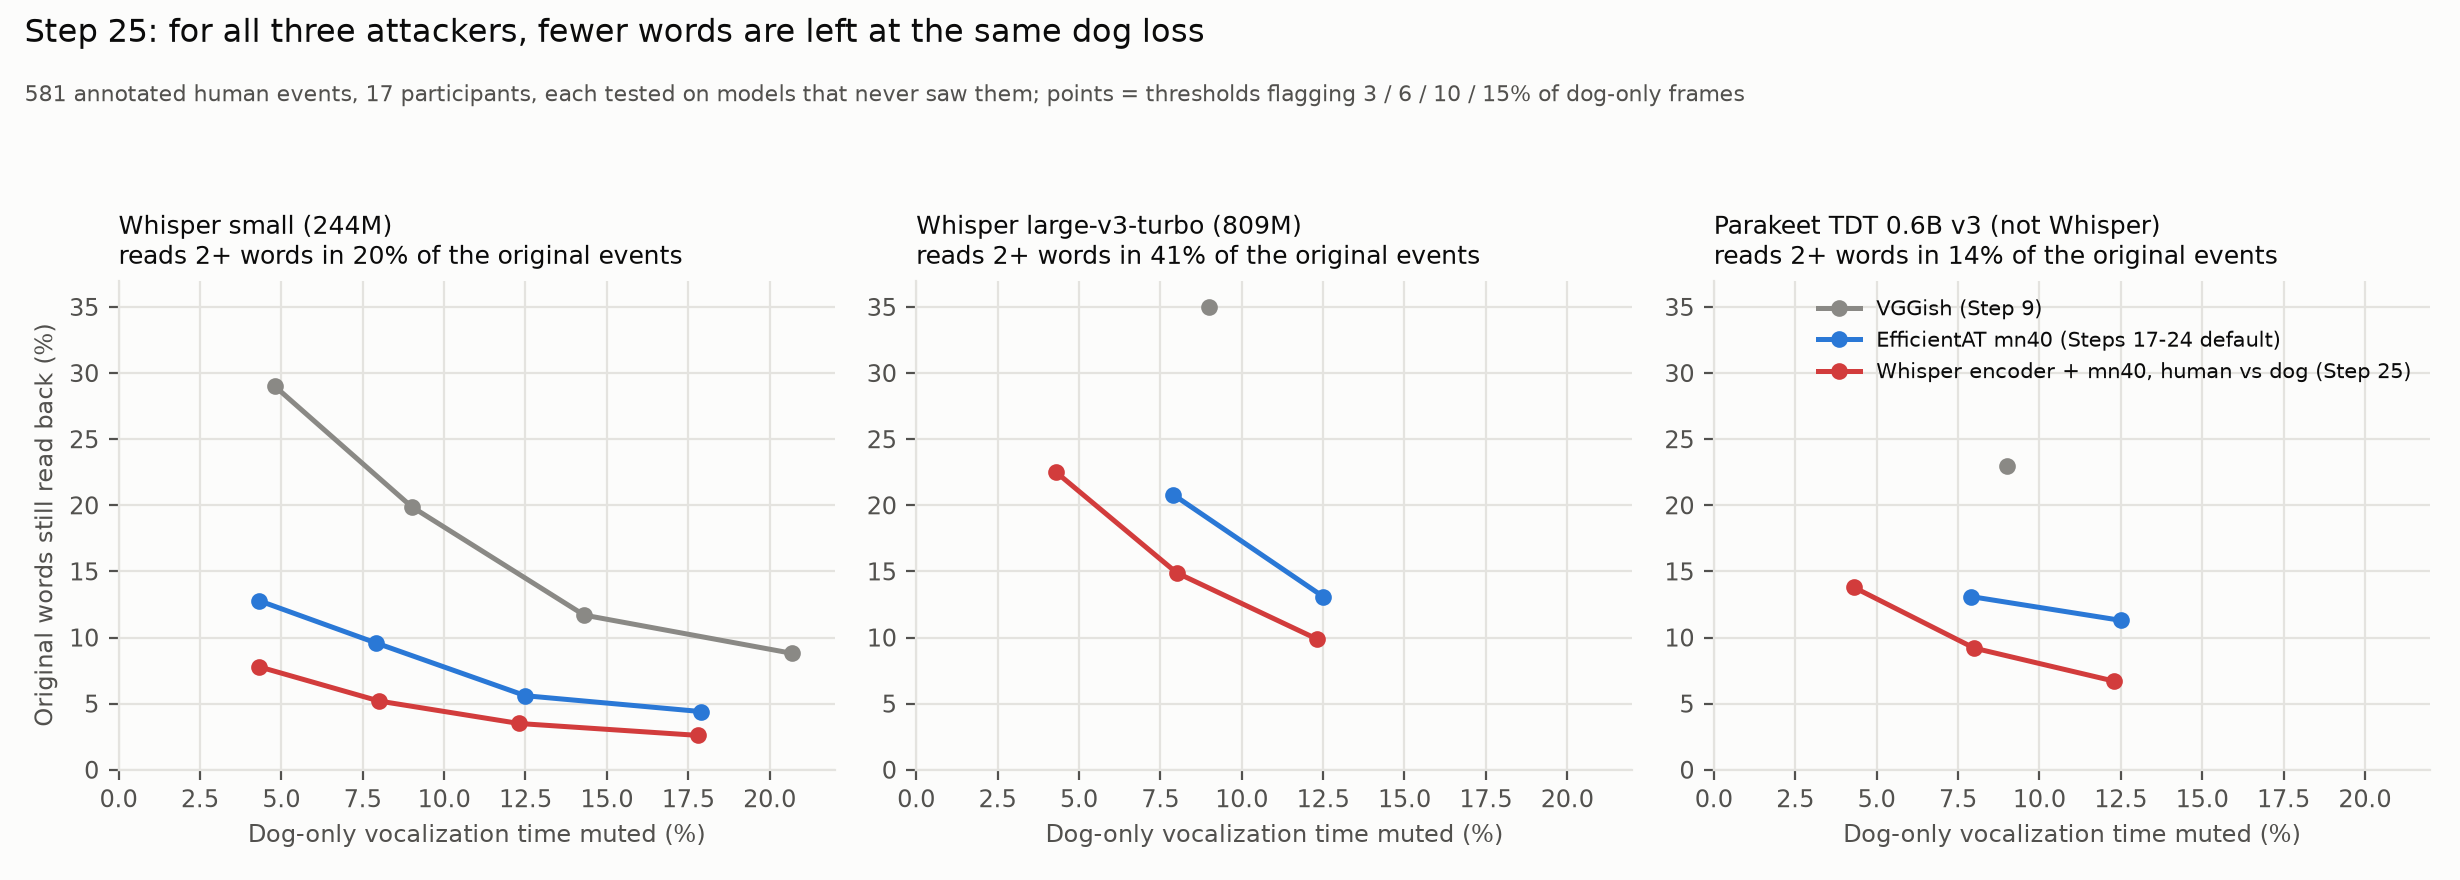
\includegraphics[width=\textwidth]{figures/step25_three_attackers.png}
\caption{Original words read back after muting, for three attackers, against the dog-only vocalization
time muted. Each line is one detector at 3/6/10/15\% of the dog-only frames flagged (turbo and Parakeet
were run at fewer points). On background audio, the share of an event's words that turn up is 0.0\%
(Whisper small, Parakeet) and 1.6\% (turbo).}
\label{fig:attackers}
\end{figure*}

\textbf{Other attackers.} Figure~\ref{fig:attackers} repeats the comparison with all three
recognizers. Parakeet, which shares nothing with the detector, reads back 9.2\% of its original words
after the new standard setting and 11.3\% after the previous one, while the dog loss drops from 12.5\%
to 8.0\%. It reads 2+ words in 2.8\% and 2.9\% of the events, below its own background floor of 4.9\%
(10 events readable only after the previous setting, 9 only after the new one). Whisper large-v3-turbo reads back 14.9\% of its words after the new
standard setting and 13.1\% after the previous one; at equal dog loss (new strict, 12.3\%) it reads
back 9.9\%. For all three attackers the new detector's curve lies below the previous one: at the same
dog loss fewer words are left. On the 29 events where Parakeet and Whisper small agree on at least two words of the original
(clearly intelligible speech), one event remains readable after the new standard setting, against
three after the previous one. The saving in dog sound therefore comes without a measurable loss of
privacy for an attacker that shares nothing with the detector.

\begin{table}[t]
\centering\small
\caption{Dog calls with no human sound on them that stay fully intact, previous vs new standard setting
(\%). Leave-one-dog-out.}
\label{tab:calls}
\begin{tabular}{@{}lrcc@{}}
\toprule
call type & events & mn40, 10\% & Whisper+mn40, 6\%\\
\midrule
pant & 1{,}116 & 71 & \textbf{82}\\
other & 243 & 75 & \textbf{83}\\
growl & 188 & 90 & \textbf{96}\\
grunt & 159 & 66 & \textbf{84}\\
bark/yelp & 48 & \textbf{75} & 67\\
moan & 32 & 62 & \textbf{75}\\
whine & 7 & 14 & \textbf{29}\\
\bottomrule
\end{tabular}
\end{table}

\textbf{Dog calls by type.} Because 89\% of the dog time is panting, the time-based cost is mostly a
panting number. Table~\ref{tab:calls} counts calls instead. The new detector leaves more calls intact
for most types: 82\% of the play pants (previously 71\%), 84\% of the grunts (66\%). Barks are the main
exception (67\% vs 75\%, 48 events): the speech encoder appears to respond to the harmonic, voice-like
bark; sneezes also lose (83\% vs 92\%, 24 events). Whines (7 events) are mostly taken for a human voice by both detectors.

\textbf{Whole recordings.} The privacy numbers cover the annotated human events. To check for speech
the annotators did not mark, Whisper read all 8\,s windows with no annotated human sound within 0.5\,s
(519 windows, 68 minutes). Ten windows produced two or more words in the unprocessed audio: eight were
typical hallucinations over dog sounds and two were short phrases worth a listen. No substantial
unannotated speech was found.

\textbf{Out of domain.} The detector was also run, unchanged and with the thresholds set on ELTE, on
40 synthetic 30\,s scenes built from material it never saw: read English speech from 20 LibriSpeech
speakers \cite{panayotov2015librispeech}, 20 ESC-50 dog clips \cite{piczak2015esc}, rooms simulated with
pyroomacoustics \cite{scheibler2018pyroomacoustics} (RT60 0.2--0.8\,s) and pink noise, with three
utterances and four dog clips per scene that partly overlap. Whisper small, scored against the reference
transcripts, reads two or more correct words in 99\% of the unprocessed utterances. After the AudioSet-only
detector it still does in 11.7\% (light) and 7.5\% (standard); after the new detector in 1.7\% and 0\%,
as after muting the exact utterances (0\%). Silero VAD \cite{silero} leaves 11.7\%. The price is dog
sound: the new standard setting mutes 57\% of the dog-only time in these scenes, against 47\% for the
AudioSet detector and 47\% for the exact utterances, because foreign barks overlap the speech and are
hard to tell from it. An earlier attempt to reach this privacy by training the AudioSet detector on
synthetic speech-under-bark scenes needed 63--77\% dog loss.

\section{What did not help}
\label{sec:negative}
\begin{itemize}\setlength\itemsep{1pt}
\item \emph{Subtracting instead of muting.} Where a dog overlaps the speech, subtracting a speech
estimate (DTLN \cite{westhausen2020dtln}, or GTCRN \cite{rong2024gtcrn} fine-tuned on this data) instead
of muting keeps some dog sound, but at equal dog loss it never left fewer readable words than muting.
\item \emph{Three microphones.} Pooling the training data of all microphones and taking the maximum
probability over them did not beat a single microphone with the same features.
\item \emph{20\,ms decisions.} About 40\% of the dog sound lost lies within 1\,s of a human sound, which
suggested finer boundaries. A classifier on every 20\,ms Whisper frame (with $\pm$0.06/0.5/1.5\,s
context, trained against all other frames) muted 68\% of the human time at 3.6\% dog loss, against 73\%
at 4.5\% for the 0.24\,s detector with the same input and objective (77\% at 7.1\% vs 81\% at 7.9\%);
interpolating the 0.24\,s probabilities to 20\,ms with tighter padding changed nothing.
\item \emph{Other inputs and labels.} Training on speech-only labels (events where Whisper reads words)
instead of all human sounds, normalizing the scores per recording, adding neighbouring frames or the
standard deviation of the Whisper frames were all equal or worse. Subtracting a separate dog detector's
score helped only with a tuned weight, and less than changing the training objective.
\end{itemize}

\section{Discussion and limitations}
The largest gains came from the input (a speech encoder) and from the training objective (human vs dog),
not from the classifier or the time resolution. The detector is a linear model on frozen features,
trained on 16 dogs in a few minutes on a laptop, and the full anonymizer, including both frozen networks,
runs at about 8$\times$ real time on two CPU cores.

The evaluation has limits. All real data come from one lab, one room and one kind of interaction; the
synthetic out-of-domain test covers other speakers, dogs and rooms only in simulation. Privacy is
measured by automatic recognizers on the annotated events; a human listening test of the remaining
readable events is still to be done. The threshold fixes the dog cost on average: at the 6\% setting
the share of dog-only frames flagged ranges from 0\% to 19\% between dogs. Handler identity is not in the
metadata, so if one person played with several dogs, the split is disjoint in dogs but not in speakers.
The inputs, objective and settings were chosen over several rounds on the same 17 folds, which makes the
best configuration somewhat optimistic; the out-of-domain test is the guard against this. Barks are muted more often by the new detector, which matters for
studies that focus on barking; the AudioSet-only detector remains available for them. Finally, muting
removes the dog sounds that overlap speech (by design); keeping those would require separating the two,
which did not work well enough here.

\section{Conclusion}
For anonymizing dog--human play recordings, a frozen speech encoder combined with AudioSet class
scores, trained on human versus dog sounds, reduces the readable speech to the level a recognizer
reaches on background noise, while losing a third less dog vocalization than an AudioSet-only detector. The code, the evaluation and a
one-command anonymizer that keeps the original file format are available at \todo{repository URL once
public}.

\section*{Acknowledgements}
\todo{The ELTE BARKS Lab for the recordings and the annotations (annotators and reviewer as listed in
the dataset metadata).}

\small
\bibliographystyle{ieeetr}
\bibliography{refs}
\end{document}
